\chapter{Exploratory Data Analysis}
\label{sec:eda}

\subsection{Introdutory Data Exploration}

\begin{figure}[H]
	\caption{The three created datasets}
	\centering
	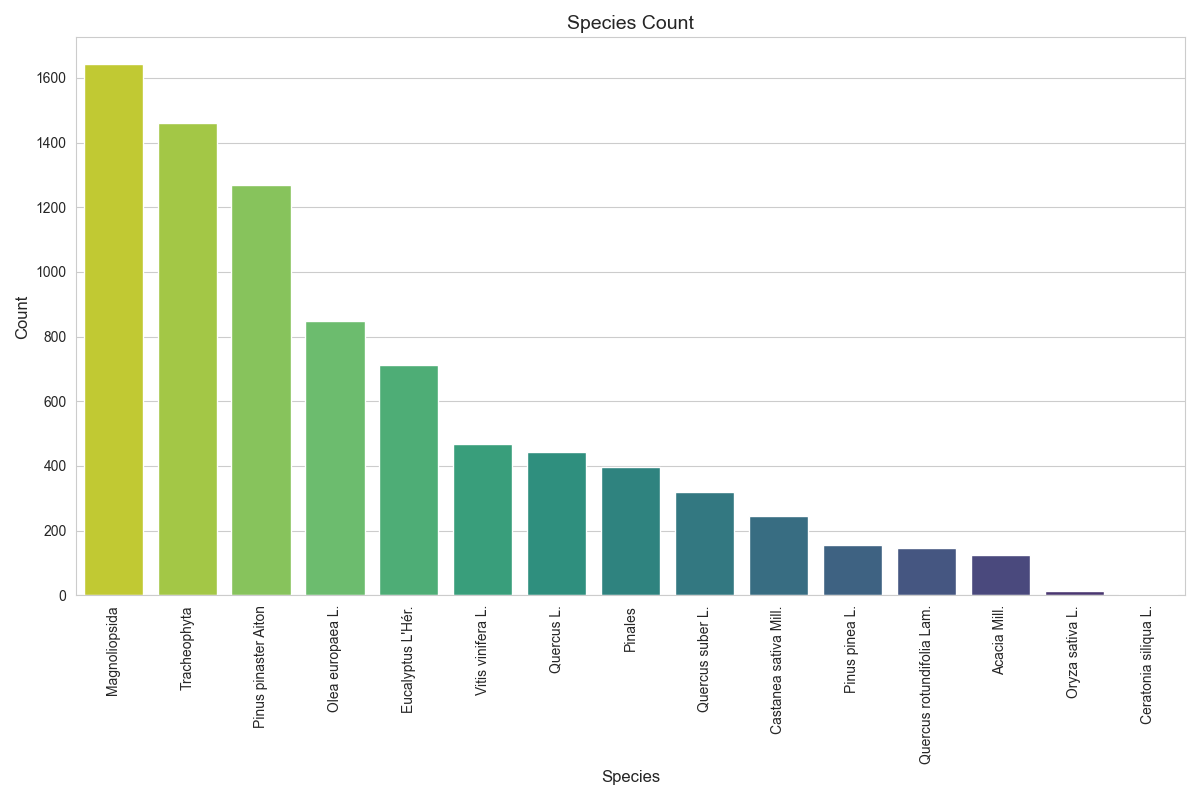
\includegraphics[width=\textwidth]{chapter-images/5_1-eda/species_count.png}
	\label{fig:species_count}
\end{figure}


Portugal's vegetation is a blend of Atlantic, European, Mediterranean, and African species \cite{britannica_portugal_climate}, and four tree species account for 80\% of all the forest area: \textit{Pinus pinaster}, \textit{Eucalyptus globulus}, \textit{Quercus suber}, and \textit{Quercus rotundifolia} \cite{Marques2011}.


\subsection{Weather variables distribution at the time of ignition}
removed variables: 'hourly.weather\_code' 'hourly.sunshine\_duration' 'hourly.is\_day' 'hourly.snowfall',
'hourly.snow\_depth', 


\begin{figure}[H]
	\caption{The three created datasets}
	\centering
	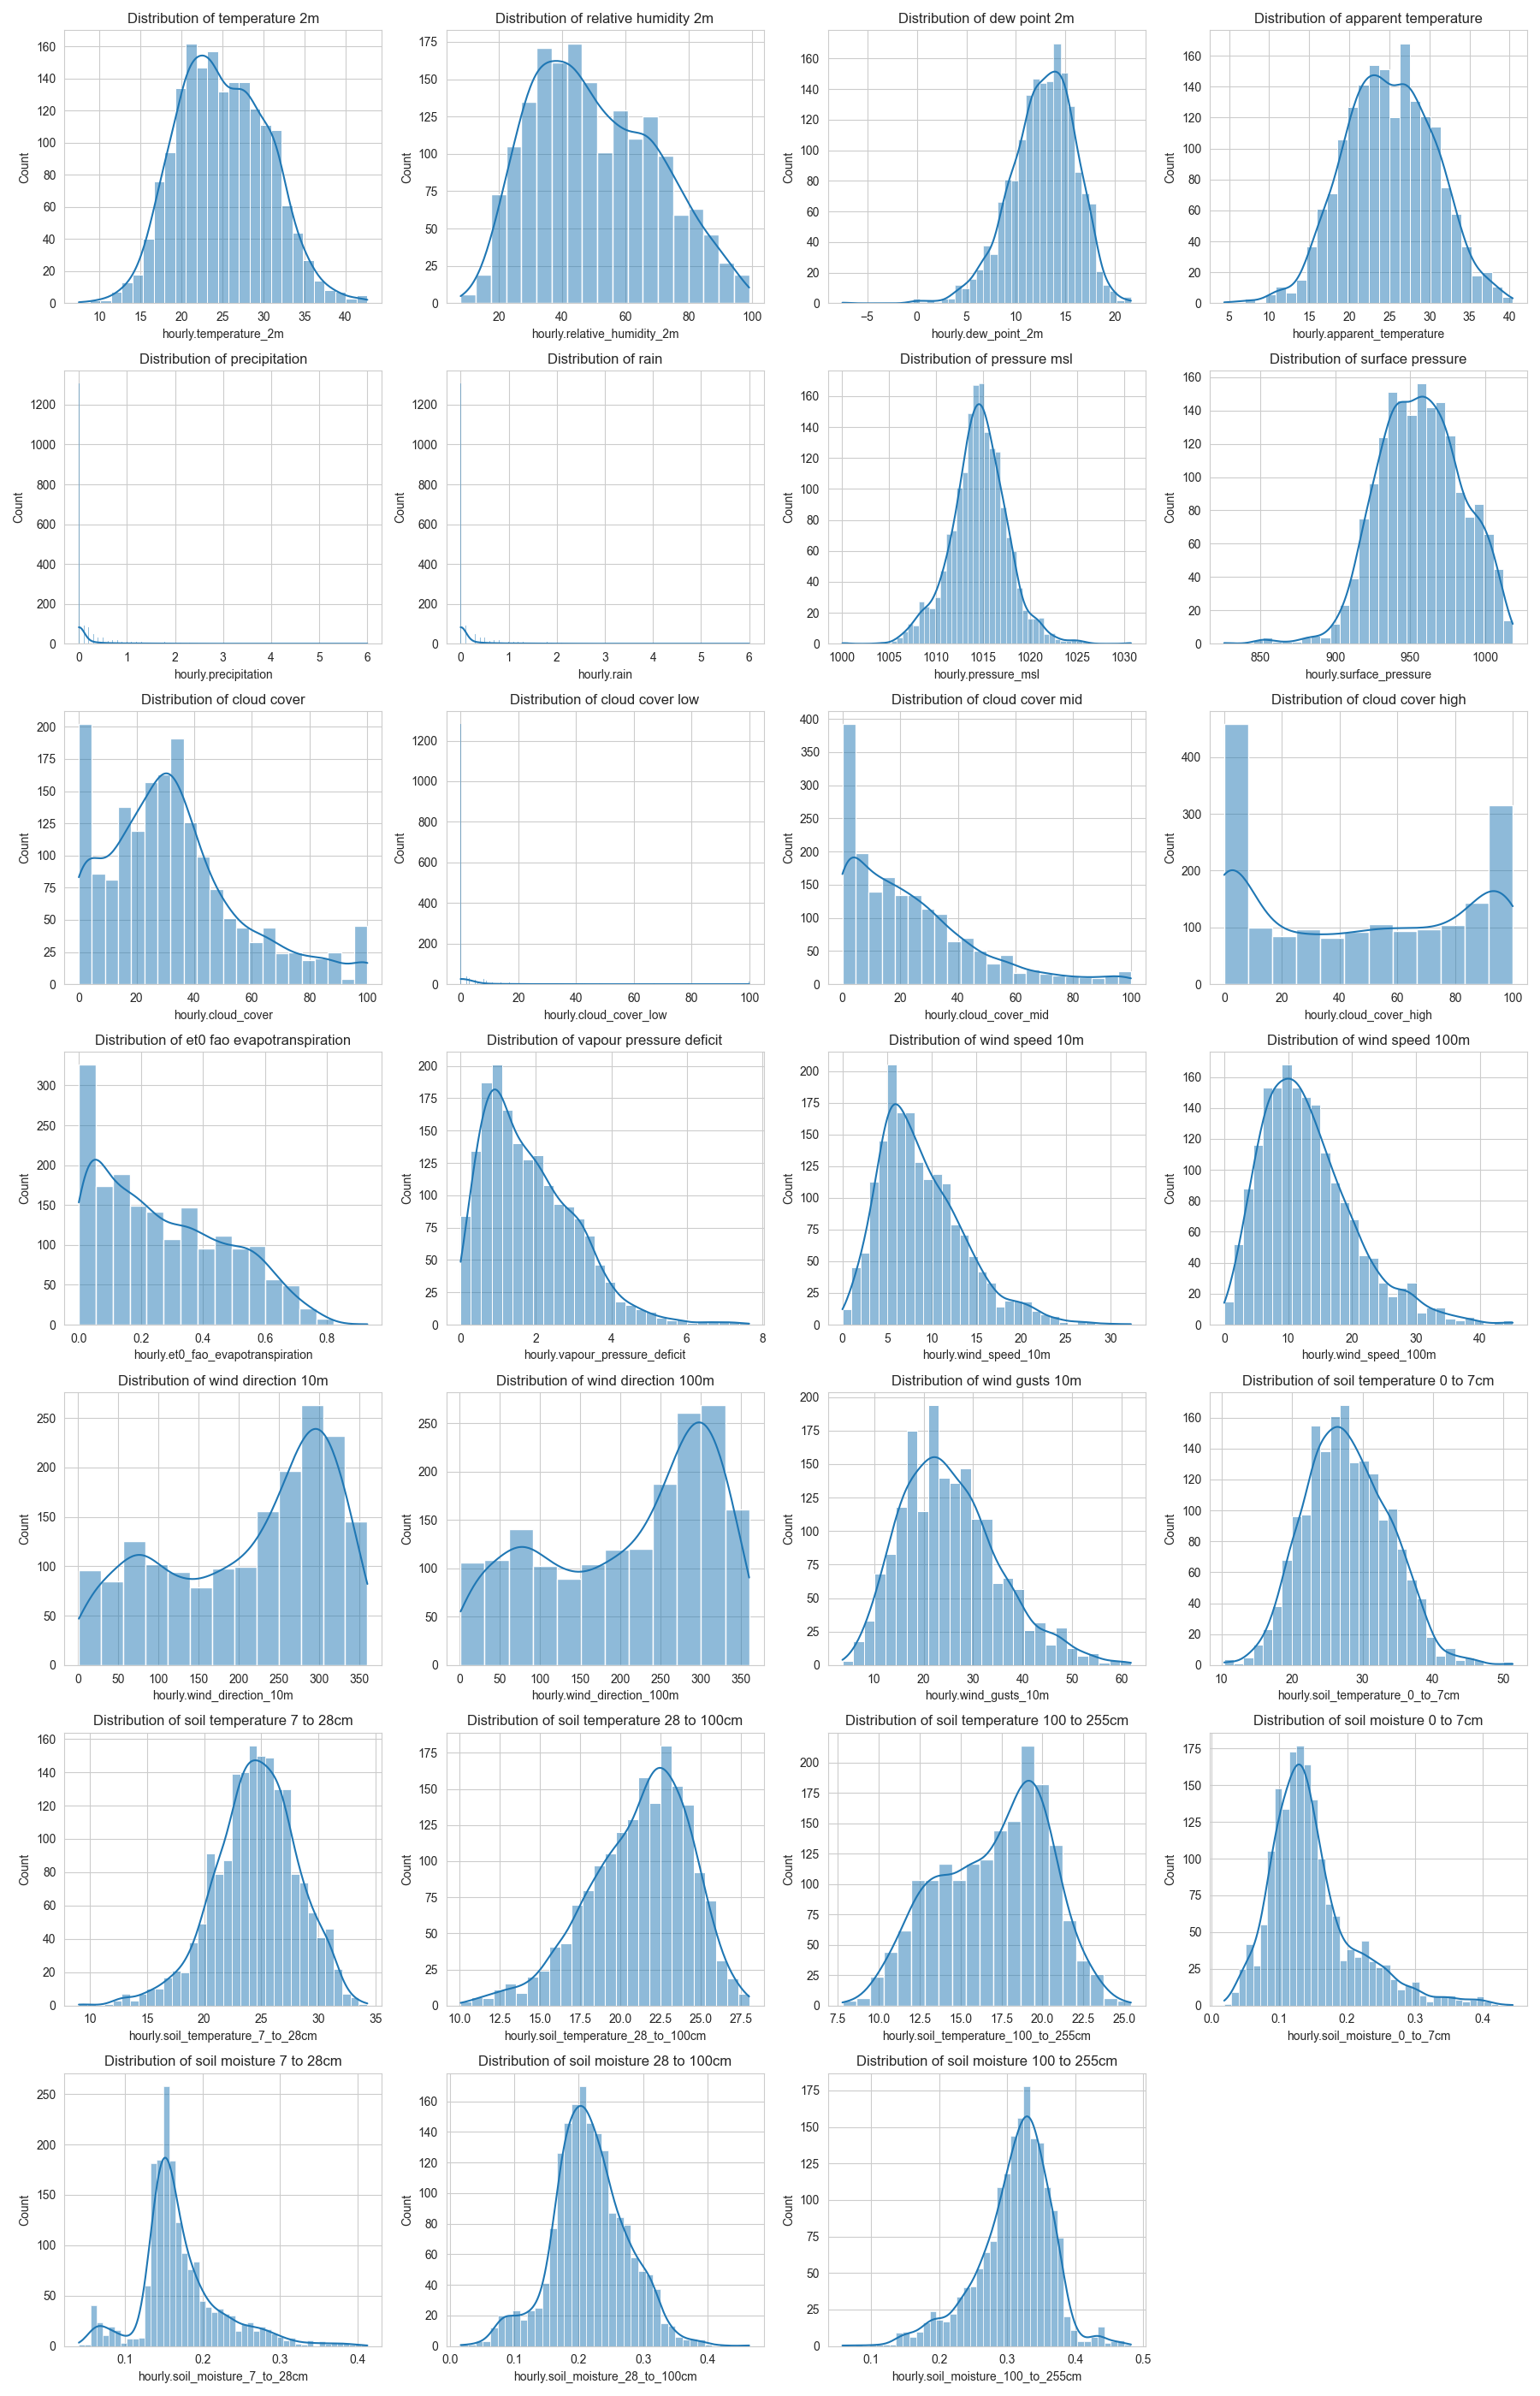
\includegraphics[width=\textwidth]{chapter-images/5_1-eda/distribution_weather_variables1FT.png}
	\label{fig:distribuiton_weather_variables}
\end{figure}

\begin{figure}[H]
	\caption{The three created datasets}
	\centering
	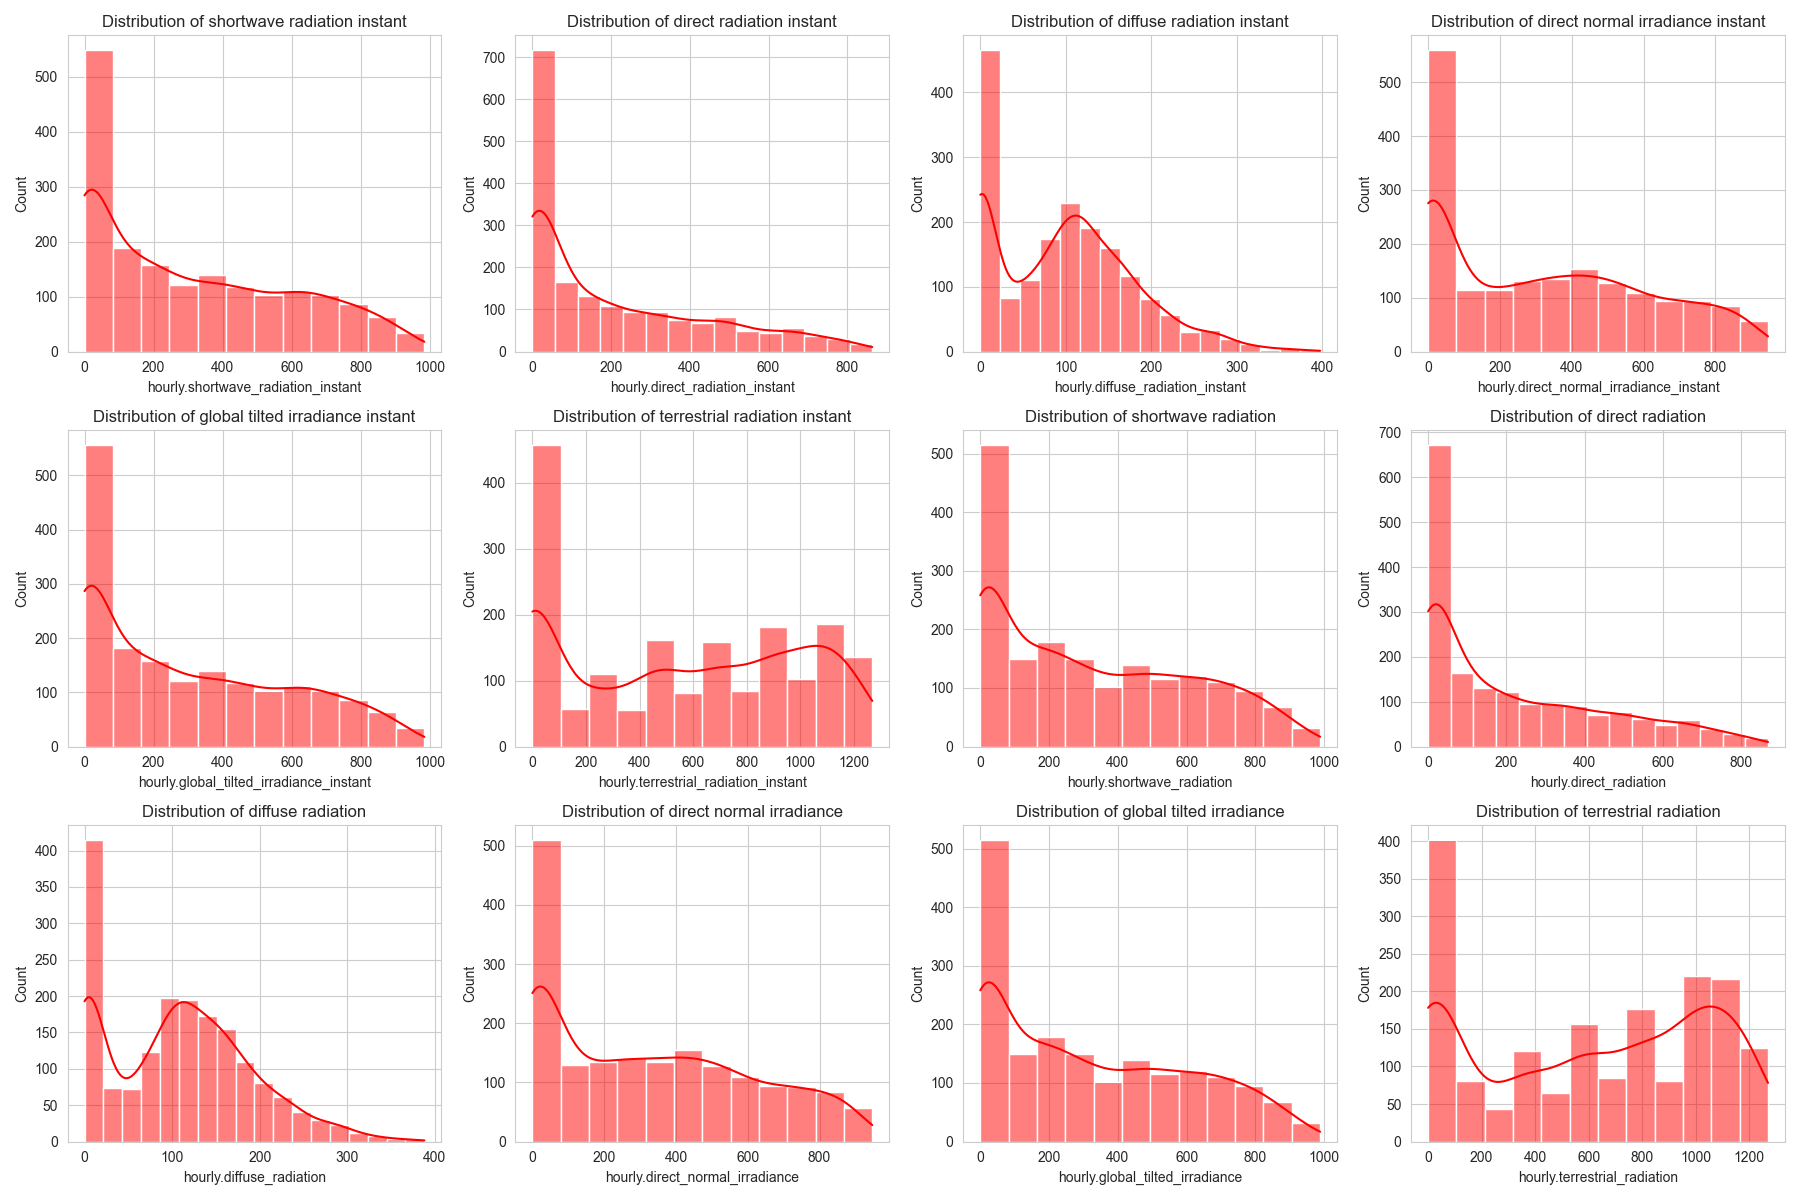
\includegraphics[width=\textwidth]{chapter-images/5_1-eda/distribution_weather_variables2FT.png}
	\label{fig:distribuiton_weather_variables_radiation}
\end{figure}

\begin{figure}[H]
	\caption{The three created datasets}
	\centering
	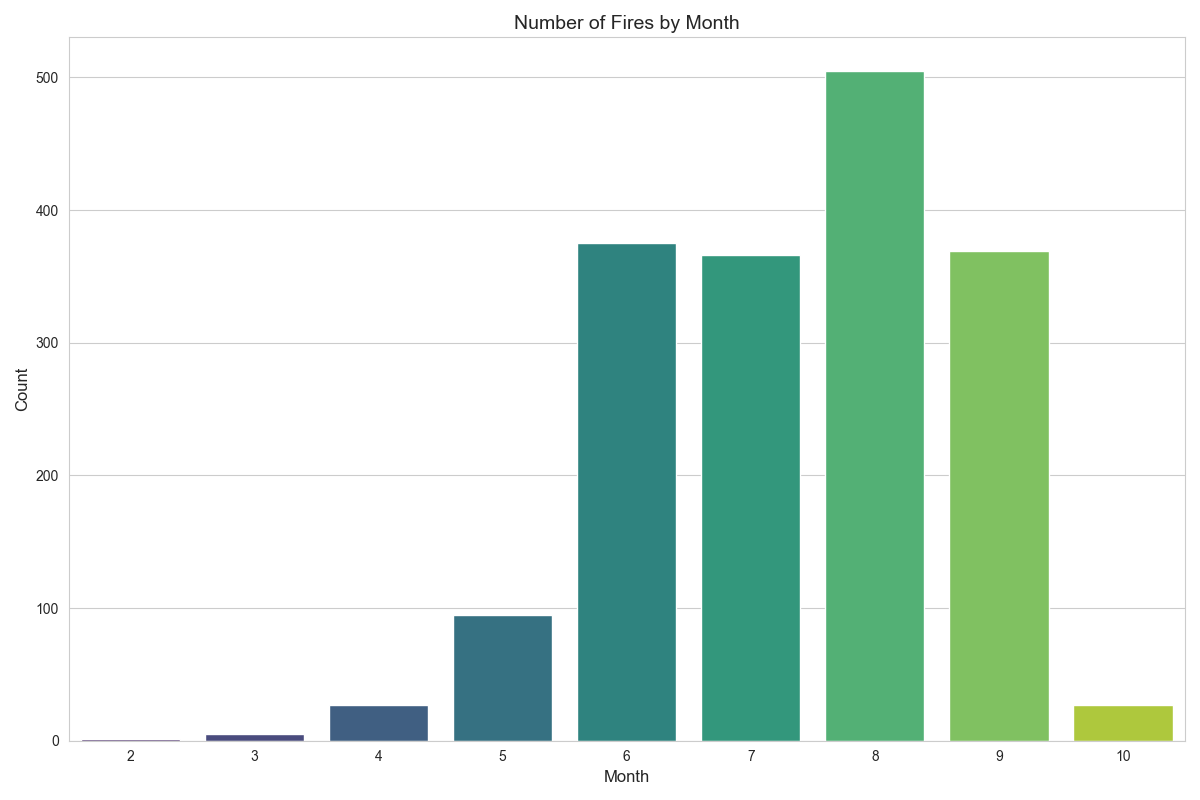
\includegraphics[width=\textwidth]{chapter-images/5_1-eda/monthly_fire_count.png}
	\label{fig:montly_fire_count}
\end{figure}



\begin{figure}[H]
	\caption{The three created datasets}
	\centering
	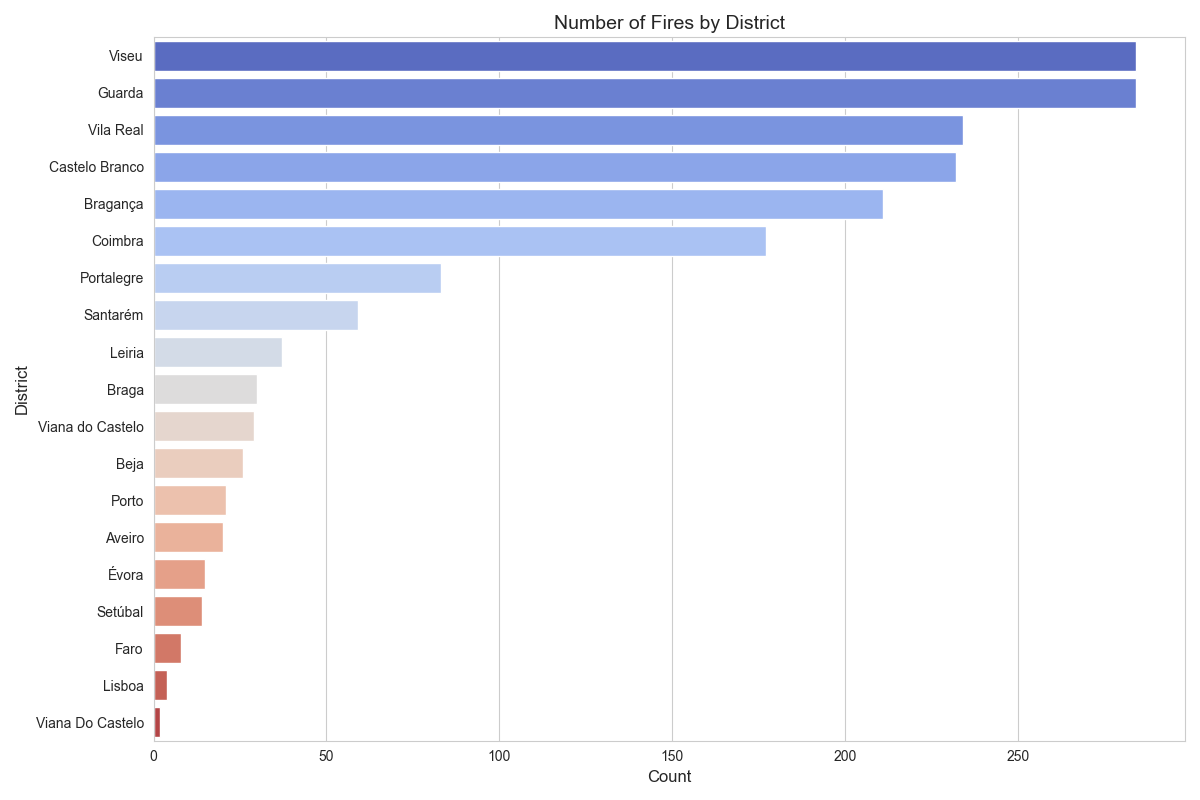
\includegraphics[width=\textwidth]{chapter-images/5_1-eda/district_fire_count.png}
	\label{fig:montly_fire_count}
\end{figure}


\begin{figure}[H]
	\caption{The three created datasets}
	\centering
	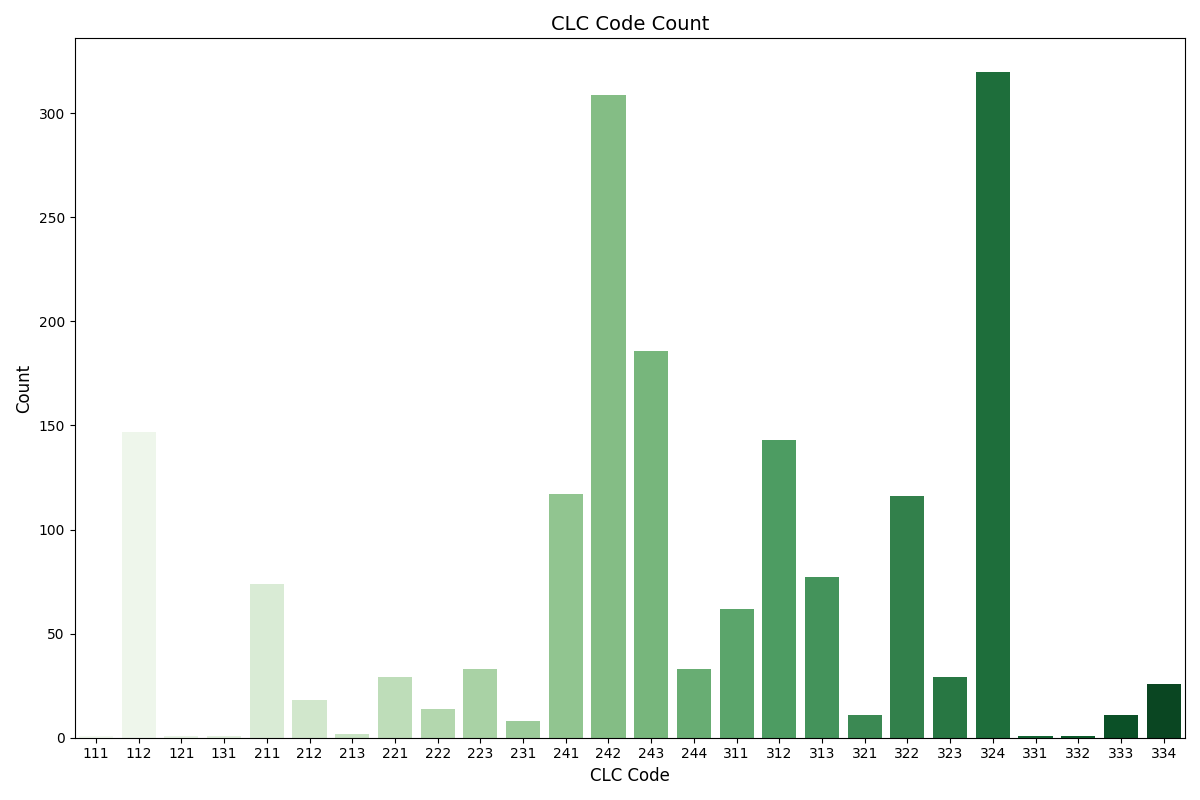
\includegraphics[width=\textwidth]{chapter-images/5_1-eda/clc_code_count.png}
	\label{fig:montly_fire_count}
\end{figure}


\section{Average conditions at ignition time}


